% !TeX root = main.tex
% !TeX spellcheck = de_DE
% !TeX encoding = utf8

\chapter{Implementation}


\section{Simulation}
For simulating the different algorithms I wrote Python scripts. I wrote an encoder using the ALT form. The encoder is a straightforward conversion of the algorithm in \cref{alt_enc_alg} into python code. The code makes heavy use of numpy and scipy for their matrix manipulation abilities. The sparse matrices from the algorithm are also stored as scipy sparse matrices to reduce the memory usage and speed up the encoding process. The overall encoding is split into two parts the offline part done only once and the ending done for every codeword. 

\subsection{Encoder}
The encoder is implemented in 2 different functions. One for the preprocessing where the parity check matrix already in ALT form is split into the required parts and $\Theta$ is inverted. The actual encoding function executes the steps from \cref{p1_steps,p2_steps}. For the sparse matrices $\bm{A}$, $\bm{B}$, $\bm{C}$, $\bm{E}$, and $\bm{T}$ the compressed sparse row matrix format from scipy is used. This format reduced the required memory significantly and accelerates the matrix vector multiplications slightly. 

\subsection{Decoder}
I wrote the decoder to represent the way I planned the FPGA implementation. So the overall structure is doing the steps that the VHDL implementation will also do. I designed it in a way that the python functions that are the core of the decoder roughly map to the VHDL entities. 

\subsubsection{Hardware Overview}
\todo{WTF is this ordering???}
I chose to reduce the hardware complexity by splitting both the check node and the variable node step each into a global calculation and a local one. The global check node calculates \cref{cn_min,cn_min2,cn_min_id,cn_sign} and the local computes \cref{cn_loc}. The same goes for the variable node where the sum over all inputs as in \cref{vn_sum} and then for the local part the input is subtracted \cref{vn_loc}.

\begin{figure}
    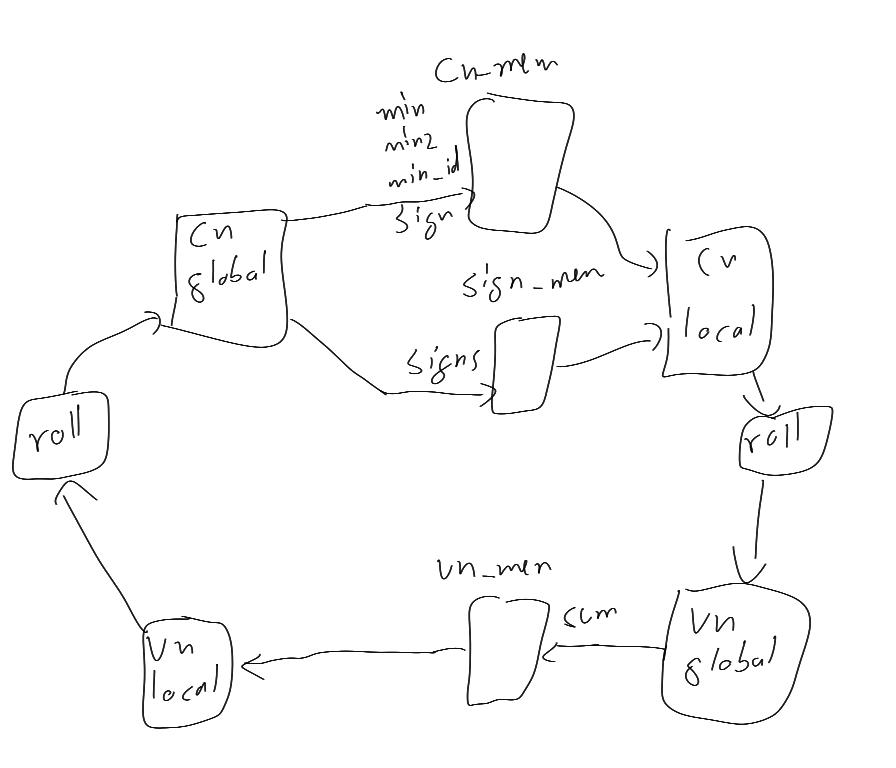
\includegraphics[width=5cm]{dataflow_circle.png}
    put the ugly paper drawing that i have all the time lying around maybe put the sizes of all dem signals here?
    \centering
    \caption{Message and Memory architecture}
\end{figure}

\todo{write something how the thing is done in vivado and u no the block stuff and how the arm cores are used and so on}

\subsection{Results}

\subsubsection{Min-sum}



\section{Hardware}
For the hardware implementation an FPGA from Xilinx is used. The device is a "ZYNQ™-7000 SOC XC7Z020-CLG484-1". It in a system on a chip consisting of a dual core ARM processor and programmable logic. The decoder is completely implemented in the FPGA logic and the encoder is software running on the ARM cores. I wrote VHDL code for the encoder.

The parameters for the hardware code were generate using Python scripts.

\subsection{Encoder}
The VHDL implementation for the encoder does the sparse matrix multiplications as fully parallel hardware. All bits are computed in parallel and no intermediate register stages are used as the encoder implemented in this way is faster than required for the decoder anyways. The sparse back substitution of $x^T = \bm{T}y^T$ is done recursively exploiting the advantages of a lower triangular matrix. Any calculation for an output only depends on the inputs and the previously calculated bits. The VHDL code is generated using Python scripts where splitting of the input matrix and the other precomputations are done with the help of numpy. I wrote a simple framework to generate the VHDL code for the matrix multiplications and back substitutions from the precomputed numpy matrices. 

\subsection{Decoder}
\todo{make some block diagramm of all my vhdl entities and their connections}
The decoder is implemented using the algorithm descibed in \cref{chap_approach}. This sections discusses how the algorithm is mapped to a hardware platform. As there are parameters that have to be optimized in oder to get decent decoding performance the decoder is designed in such a way that it is easy to change parameters as for example the bit width of the stored values or the used parity check matrix. 

Overall the decoder is written in VHDL but on file containing definitions for all signals and the decoder state machine is autogenerated with a python script. In this script it is possible to change the bitwidth of the LLRs and the parity check matrix.

The decoder is controlled by a state machine which reads the "instruction list" and outputs the control signal and the memory read and write addresses. This instruction list is also created by the decoder python script. There it is also possible to change the clock cycle in which each signal appears. This makes it easy to change the pipelining. \cref{datafl_tree} shows how the message LLR values are passed along the entities. Each iteration of the decoder is split into two parts. The first part calculated the global check nodes results and the second part the global variable node results.

I will start with the global variable node pass as this has fewer steps and some of the steps are reused in the check node pass. First the local check node results are calculated. This is done from the stored minimum, second minimum, minimum id, and the signs. The output is either the minimum if the minimum id is not equal to the current position or otherwise the second minimum. The sign for this output is taken from the sign input, as all minimums are absolute values. Now the messages are passed through a barrel roll to shift the values to the appropriate positions. The rolled value is then accumulated for each column and at the end of the column stored. 

The global check nodes pass starts the same as the global variable node one until the barrel roll. After rolling the LLRs are passed into the local variable node entity. The local variable node subtracts the incoming LLR from the sums the variable nodes calculated and outputs it. Now the LLRs are passed through a reverse roll to align them for the global check node. The global check node then does an accumulation. This consists of taking the minimum, second minimum, and the signs for the minimum. Also the signs of all incoming LLR values are output.

\begin{figure}
    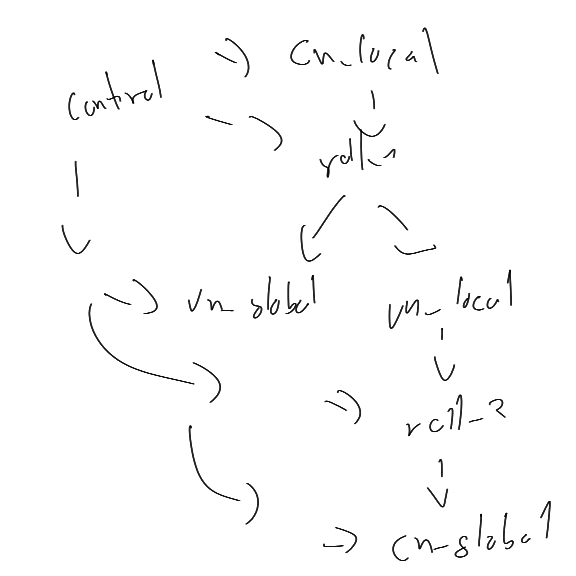
\includegraphics[width=5cm]{dataflow_tree.png}
    maybe add the min mangle at the end
    \centering
    \caption{Dataflow Diagram of the Decoder}
    \label{datafl_tree}
\end{figure}

\subsection{Control}
The decoder is controlled by a state machine which reads the addresses for the memory and all control signals from a ROM. It als keeps track of the number of iterations already done and terminates if the iteration number reaches a specified maximum. Additionally the state machine stops the decoding process if the output vector is error free. The instructions consisting of addresses and control signal are generated by the Python script which also generates the other constants. 

\subsection{Check Nodes}
As the check nodes are split into two steps I wrote two separate entities executing these operations. One is the local check node, computes the message LLR from the minimums, minimum sign, and LLR signs. From the controller it receives the current offset. 

\begin{figure}
    LLR from min schematic maybe?
    \centering
    \caption{Schematic Diagram of a Local Check Node}
\end{figure}

\begin{figure}
    min entity schematic maybe?
    \centering
    \caption{Schematic Diagram of a Global Check Node}
\end{figure}

\subsection{Variable Nodes}
Also the variable nodes are split into two. The global pass sums all the incoming LLR values and at the end of each column it is stored into memory. The local check node retrieves these sums and calculates
\begin{equation}
    q_{nm} = S(n) - r_{mn}
\end{equation}
, where $S(n)$ is the stored column sum, $r_{mn}$ and $q_{nm}$ are the incoming and outgoing LLRs respectively.

\subsection{Barrel Roll}
I started first with a naive implementation for the barrel roll
\begin{lstlisting}[style=vhdl]
    entity dynamic_roll_sign is
	generic (
		DIRECTION : boolean --true means the same direction as fixed roll
	);
    port (
		roll_count : in unsigned;
        data_in : in min_signs_t;
		data_out : out min_signs_t
    );
end entity;

architecture base of dynamic_roll_sign is
begin
    gen_i : for i in data_in'range generate
    begin
        data_out(i) <= data_in((i - to_integer(roll_count)) mod data_in'length) when not DIRECTION 
            else data_in((i + to_integer(roll_count)) mod data_in'length));
    end generate;
end architecture;
\end{lstlisting}
but this generates huge hardware. The primary problem is the synthesis generates a division to implement the modulo operations. In the following I will show that the modulo can in this case be replaced by a conditional addition or subtraction. But first I have to set some limits for the inputs. The input has to be in the range $0 \leq$ \lstinline{roll_count} $<$ \lstinline{data_in'length}. From that I know 


\subsection{Possible Improvements}
More pipelining
In and output double buffering
More pipeline stages
u no dependency optimization
